\documentclass[12pt, onecolumn,notitlepage]{scrartcl}
%\documentclass[handout]{beamer}
%\documentclass[draft]{beamer}


\usepackage[utf8]{inputenc}
\usepackage[T1]{fontenc}
\usepackage[english, ngerman]{babel}
\usepackage{graphics} %Für Bilder
\usepackage{graphicx} 
\usepackage{colortbl}
\usepackage{adjustbox}
\usepackage{float}
\usepackage{csquotes}
\usepackage{amssymb}
\usepackage{amsmath}

\restylefloat{table}

\bibliographystyle{ieeetr}

\begin{document}

\title{Verteiltes System zur Berechnung der Mandelbrotmenge}

\author{Lars Klee, 1288210\\Randy Stoppe, 1390338\\Josua Kirsch, 1293138\\Universität Trier}
\date{Trier den \today}

\newcommand{\define}[1]{\color{darkorange}Definition: \color{black}{#1}\\  } 



\maketitle
\tableofcontents


\section{Einleitung}
Diese Arbeit entsteht im Rahmen des großen Studienprojektes bei der Professur Systemsoftware und Verteilte Systeme der Universität Trier.
\subsection{Motivation}
\subsection{Problemstellung}
Die Mandelbrotmenge ist die Menge der komplexen Zahlen $c$, für die die durch die Iteration \begin{gather}
z_{ 0 } = 0  \\
z_{ n+1 } = z_{ n }^{ 2 } + c
\end{gather}
definierte Folge $(z_{ n })_{ n\in \mathbb{N} }$ beschränkt ist. Diese lässt sich auf der komplexen Ebene geometrisch interpretieren und bildet ein Fraktal. Wird jedem Punkt auf der komplexen Ebene ein Pixel mit dem entsprechenden Wert von $c$ zugewiesen, ergibt sich eine graphische Darstellung der Mandelbrotmenge. Liegt ein Punkt in der Mandelbrotmenge, so wird ein Pixel schwarz gefärbt, liegt er nicht in ihr, so hängt seine Farbe davon ab, wie schnell die Folge mit dem betreffenden $c$ gegen Unendlich strebt. Diese Berechnung ist äußerst rechenintensiv, jedoch kann jeder einzelne Pixel unabhängig voneinander berechnet werden. Somit bietet sich eine Berechnung der Mandelbrotmenge durch ein verteiltes System an.
\subsection{Zielsetzung}
Das Ziel dieser Arbeit ist es, ein verteiltes System zu entwickeln, welches in der Lage ist, die Mandelbrotmenge und dessen Zoomstufen performant zu berechnen. Zu diesem Zweck wird ein Server in Java programmiert, zu dem sich Clients verbinden und Rechenaufträge zur Berechnung der Mandelbrotmenge erhalten können. Der Server selbst rechnet dabei keinen einzigen Punkt der Mandelbrotmenge aus sondern empfängt die errechneten Ergebnisse der Clients und stellt diese daraufhin graphisch dar. Über die Nutzeroberfläche kann in die Mandelbrotmenge herein- und herausgezoomt werden, wodurch neue Rechenaufträge verteilt werden.  \par
Die unterschiedlichen Clients werden jeweils unter unterschiedlichen Technologien programmiert. So wird der erste Client als Android-Anwendung entwickelt, der zweite Client als CUDA-Anwendung unter Zuhilfenahme des Grafikprozessors und der dritte Client als browserbasierte Anwendung mit JavaScript und WebAssembly. 
\subsection{Gliederung}
Die folgenden drei Kapitel beschreiben jeweils einen der entwickelten Clients und enthalten jeweils Unterkapitel, die die zugrundeliegenden Technologien, die Bedienung und letztlich die Entwicklung der Clients sowie der Probleme, die in dieser auftreten, beschreiben. Darauf folgt eine Dokumentation des Servers, die dessen Funktionsweise näher erläutert. Schlussendlich erfolgt eine Reflexion, in der sich damit auseinandergesetzt wird, inwiefern die Zielsetzung erfüllt werden konnte und ob die Verwendung der jeweiligen Technologien sich als Vorteil erwiesen hat oder nicht.


\section{Android Client}
\subsection{Verwendete Technologie}
Bei der App-Programmierung kann zwischen Kotlin, Java und C++ als Programmiersprachen gewählt werden. Hier wird C++ zur Berechnung der Mandelbrotmenge und Java für die Server-Client-Kommunikation, Button-Listener und zur Überprüfung der WLAN-Verbindung verwendet. Das eigentliche Hauptproblem bei Android oder im Generellen bei Smartphones ist, dass diese, im Gegensatz zu PCs, beschränkte Ressourcen vorweisen, sei es CPU-Leistung, RAM, Speicherplatz oder Batterielaufzeit. Auch wenn diese Beschränkungen mit neuen Modellen und Technologien immer weiter abnehmen, sollte dennoch dafür gesorgt werden, dass die App möglichst Ressourcen schonend programmiert wird. Außerdem muss bei der App-Programmierung dafür gesorgt werden, dass der der main-Thread, auch UI-Thread genannt, möglichst wenig Arbeit auszuführen hat, da dieser, wie der Name bereits andeutet, dafür verantwortlich ist, dass die UI weiterhin auf Eingaben reagieren kann. Wenn dieser Thread zu viel Arbeit verrichten muss, dann kann es nach einer gewissen Zeit zu einer ANR-Meldung (Application Not Responding) kommen, dann bekommt der Nutzer die Möglichkeit die App zu beenden oder zu warten, bis die Aufgabe beendet wurde und die UI auf eine Eingabe reagieren kann. Deswegen ist in der App-Programmierung wichtig, so wenig wie möglich auf dem UI-Thread laufen zu lassen. Dies war zu Beginn des Projekts ein Problem, da immer wieder dem UI-Thread zu viele Aufgaben gegeben wurde und die App regelmäßig abstürzte. Man muss sehr viel in neue Threads auslagern, wie zum Beispiel der Verbindungsaufbau zum Server, aber auch das Verschicken einer einzelnen Nachricht, da sonst die App mit der Fehlermeldung „NetworkOnMainThreadException“ abstürzt.
\subsection{Bedienungsanleitung}
\subsubsection{Starten der Anwendung}
\subsubsection{UI-Erklärung}
Wenn man die App startet und man den Startbildschirm  sieht, dann hat der User die Möglichkeit am oberen Bildschirmrand einen Namen für das Gerät einzugeben, dieser wird mit an den Server geschickt und der Androidsocketthread erhält dann diesen Namen damit man, wenn die Verbindung beendet wird, besser erkennen kann bei welchem Client die Verbindung beendet wurde. Darunter besteht die Möglichkeit die gewünschte IP-Adresse  sowie den Port  des Servers einzugeben. Entsprechen die Eingaben den Wünschen so kann mit einem Klick auf Connect   versucht werden eine Verbindung zum Server herzustellen, wenn dies nicht gelingt so bekommt der User eine Rückmeldung per Toast-Nachricht woran es gelegen hat (Server nicht erreichbar, keine WLAN-/Internetverbindung, ungültige IP/Port). Wenn der User alle Eingaben verwerfen will, so besteht die Möglichkeit mit einem Klick auf den Delete-Button  dies zu ermöglichen. \par
Wenn eine Verbindung zum Server aufgebaut werden konnte so wechselt die Ansicht zum Berechnungsbildschirm. Dort kann der User am oberen Bildschirmrand die CPU-Usage sowie die Memory-Usage einsehen. In der Mitte des Bildschirms kann die Network-Usage  eingesehen werden. Diese zeigt an wie viele kb/s gesendet bzw. empfangen werden, daran kann man erkennen ob gerade ein Datenaustausch zwischen Client und Server stattfindet. Über den Buttons wird der zuvor auf der Startseite eingegebene Gerätename angezeigt. Im unteren Drittel des Bildschirms werden die Buttons dargestellt. Am unteren Ende des Bildschirms hat der User die Möglichkeit den aktuellen Status, ob eine Berechnung läuft oder pausiert ist, einzusehen. Mit einem Tippen auf Start fragt der User die erste Task an und wird berechnet daraufhin, bis pausiert oder beendet wird, die Mandelbrotmenge, außerdem wechselt der Text auf dem Button zu „Running…“). Mit einem Klick auf Pause wird die aktuell laufende Berechnung beendet und an den Server geschickt, aber keine neue Task angefordert, dies kann wieder fortgesetzt werden wenn der User wieder auf den Start-Button, der jetzt die Beschriftung „Resume“ hat, klickt. Der Pause-Button wechselt, nachdem er geklickt wurde, seine Beschriftung von „Pause“ auf „Paused“. Wenn man die Berechnung wieder fortsetzen möchte, dann kann man auf den Start-Button, jetzt mit der Beschriftung Resume, tippen anschließend wird die Berechnung der Mandelbrotmenge fortgeführt. Mit einem Klick auf \enquote{Quit} wird die Verbindung zum Server getrennt, falls eine Berechnung laufen sollte, dann wird der User gefragt ob er die laufende Berechnung unterbrechen will oder nicht. Wenn der User auf \enquote{Quit} klickt und gegebenenfalls die Berechnung beendet, dann wechselt die Ansicht wieder zum Startbildschirm.


\subsection{Entwicklung \& Probleme}
Zu Beginn sollte die App nur den von der App selbst benutzten RAM anzeigen lassen, dies erwies sich schwieriger als gedacht, denn jede App bekommt vom System eine bestimmte Menge an RAM zur alleinigen Verfügung gestellt, allerdings benutzen die Apps auch sogenannten „shared Memory“ und dieser wird von mehreren Apps benutzt, was die Bestimmung der Menge des benutzten RAMs für eine bestimmte App erschwert. Aus diesem Grund wird die Gesamtmenge an belegtem RAM angezeigt um so dann ableiten zu können ob die App richtig arbeitet. \par
Nach ersten Recherchen hätte man das Smartphone „rooten“ müssen um die benötigten Informationen auslesen zu können, damit die CPU-Usage ausgelesen und somit angezeigt werden kann. Dies ist allerdings nicht zu empfehlen, da nach diesem Vorgang im schlimmsten Falle das Smartphone nicht mehr benutzbar ist. Außerdem können integrierte Sicherheitssysteme nach dem Root-Vorgang nicht mehr aktiviert werden und dadurch wird das Smartphone anfälliger für Virus- oder Malware-Angriffe. Aus diesen Gründen wurde zunächst auf das Rooten und auf das Anzeigen der CPU-Usage verzichtet. Nach weiteren Recherchen wurde eine Lösung, ohne das Smartphone rooten zu müssen, auf den folgenden Internetseiten gefunden:
\begin{itemize}
	\itemsep0pt
	\item http://www.java2s.com/Code/Android/Hardware/GetCPUFrequencyCurrent.htm
	\item http://www.java2s.com/Code/Android/Hardware/GetCPUFrequencyMin.htm
	\item http://www.java2s.com/Code/Android/Hardware/GetCPUFrequencyMax.htm 
\end{itemize}

Aus diesen drei Links wurde dann die gewünschte Lösung abgeleitet (siehe „CpuInfo.java“).\\
Das Anzeigen der Network-Usage hat von Beginn an zufriedenstellend funktioniert und dient dazu um zu überprüfen ob eine Kommunikation zwischen dem Client und dem Server stattfindet.\\
Nachdem das Anzeigen der Auslastungen jetzt zufriedenstellend funktioniert und der Verbindungsaufbau vom Client zum Server in einen extra Thread ausgelagert worden ist und somit eine Verbindung hergestellt werden kann, konnte sich nun der Berechnung der Mandelbrotmenge und der Versendung der Ergebnisse an den Server gewidmet werden. Die Kommunikation zwischen Client und Server geschieht mittels TCP. \par
Übertragung zwischen Client und Server (Version 1.0): 
Der Client hat zu Berechnung alle benötigten Variablen vom Server erhalten (wie genau siehe Dokumentation zu Server-Version 1.0). Anschließend hat der Client mit einem Klick auf den Start-Button die Berechnung gestartet. In Version 1.0 hat der Client allerdings jeden Pixel des Bildes einzeln an den Server geschickt, dies führte zu einer langen Laufzeit um nur das Startbild zu berechnen und auf der Serverseite darzustellen.\par
Mit dem Wechsel zu Server-Version 2.0 sind diese Probleme behoben, da jetzt eine komplette Zeile zunächst auf der Clientseite berechnet wird und dann anschließend an den Server verschickt wird und somit eine Zeile auf der Serverseite dargestellt werden kann. Bei Version 2.0 berechnet jetzt ein Client nicht mehr einen bestimmten Bereich des Bildes sondern fragt jetzt immer nach einer berechneten Zeile eine neue Task an. Dies hat dafür gesorgt, dass die Zeitdauer um das Startbild darzustellen verkürzt wurde (mehr zur Zeitdauer weiter unten). Beim Erhalten der Taskwerte kam es allerdings auf Clientseite zunächst zu Problemen, da die Werte vom Server als Byte-Array mittels DataOutputStream verschickt wurden aber auf Clientseite mithilfe eines BufferedReaders als String eingelesen wurden und dann bei der Umwandlung von String in Byte-Array Fehler auftraten wie zum Beispiel, dass das Empfangene Byte-Array eine falsche Länge aufwies und somit konnte der übermittelte Wert nicht aus dem Array generiert werden. Die Lösung dieses Problems ist es nach dem Erhalt der Task-Nachricht, welche dem Client signalisiert, dass die nächsten Nachrichten, die geschickt werden, die Werte sind, die benötigt werden um eine Zeile der Mandelbrotmenge zu berechnen, mithilfe eines DataInputStreams die Nachrichten einzulesen. Außerdem werden die Werte vom Server nicht mehr als Byte-Array sondern als int für den x- und itr-Wert bzw. als double für den xMove-, yMove- und zoom-Wert verschickt und auf Clientseite mit readInt() bzw. readDouble() vom DataInputStream eingelesen. Nun kann die Mandelbrotmenge erfolgreich berechnet werden, allerdings kam es zunächst zu Problemen, da die Übermittlung der in C++ berechneten Punkte, also einer ganzen Zeile, zu Java nicht richtig funktioniert hatte, dies wurde behoben indem zunächst die initializePackage-Methode in Reader.java angepasst wurde. Diese Methode wurde in C++ aufgerufen und es wurden der x-, y- und itr-Wert nach jedem for-Schleifendurchlauf übergeben und in Reader.java zu einem String zusammengefasst. Diese Methode wurde im späteren Verlauf durch die format-Methode in C++ ersetzt, nun wird nur das komplette Paket von C++ an Java übergeben. Jetzt kam es allerdings zu dem Problem, dass die Berechnung in der while-Schleife in eine Endlosschleife gelang, da in der Abfrage versehentlich „itr>0“ und nicht „tmp>0“ abgefragt wurde. Nachdem ein Paket jetzt erfolgreich erstellt und an den Server geschickt wird, warf der Server eine NoSuchElementException, dies lag daran, dass die letzten beiden Zeilen eines Paktes wie folgt aussahen: \\
... \\
„\textbackslash n“ \\
„\textbackslash ntick“ \\
Die Exception wurde geworfen als der Server den Zeilenumbruch eingelesen hatte. Dieses Problem konnte gelöst werden, in dem „\textbackslash n“ entfernt wurde. Solange der Pause-Button nicht geklickt wurde, wird an jedes Paket eine Zeile mit dem Inhalt „\textbackslash ntask“ angefügt. Diese sorgt dafür, dass der Server dem Client eine neue Task zuschickt. \par
Jetzt kann der Client erfolgreich Tasks entgegennehmen, diese berechnen und an den Server zurückschicken und dieser kann die Pakete dann erfolgreich darstellen. Jedoch warf der Server jetzt eine StackOverflowException, dies lag daran, dass bei der sendTask-Methode des Servers nach dem Verschicken des Iterationswerts nochmal recieveMessage() aufgerufen wurde obwohl dies allerdings unnötig war und somit gelöscht werden konnte und somit das Problem gelöst hat. \par
Die Check-Klasse sorgt dafür, wenn die Internetverbindung abbricht oder zu schwach ist, dass dann die Verbindung zum Server getrennt wird und die Ansicht auf dem Bildschirm wieder zum Startbildschirm wechselt. Zunächst wechselte die Ansicht nicht zum Startbildschirm zurück, wenn die WLAN-Verbindung unterbrochen wurde, da bei der Überprüfung welches Fragment, also welcher Ansicht gerade aktiv ist, ein Fehler unterlaufen ist. Mithilfe des FragmentManager konnte dieses Problem gelöst werden, denn fragmentManager.getPrimaryNavigationFragment() liefert das aktuelle aktive Fragment und somit kann der Befehl \\
\textit{NavHostFragment.findNavController(Objects.requireNonNull(fragmentManager\\.getPrimaryNavigationFragment())).navigate(R.id.action\_secondFragment\_to\\\_firstFragment)} \\
erfolgreich ausgeführt werden. Das gleiche Problem trat auch beim Tippen auf den Quit-Button auf und konnte genauso gelöst werden. \par
Durch Zufall fiel auf, dass im Logcat, wenn man zur zweiten Ansicht wechselt, zwischen 30 und 40 Frames jede Sekunde übersprungen werden, da der UI-Thread zu viel Arbeit verrichtet. Das liegt vermutlich daran, dass jede Sekunde die CPU-Usage, Memory-Usage sowie die Network-Usage aktualisiert werden und dieser Vorgang muss auf dem UI-Thread laufen, da dieser der einzige ist der die UI aktualisieren kann. Die Benutzeroberfläche reagiert allerdings noch auf jede Eingabe und somit stellt dies kein schwerwiegendes Problem dar und kann ignoriert werden.
Ein weiteres Problem besteht darin, dass, nachdem die App beendet wird und das Smartphone mit dem PC mit einem USB-Kabel wieder verbunden wird sowie Android Studio neugestartet wird, weiterhin Ausgaben im Logcat stattfinden. Es können allerdings keine neuen Berechnungen sein, da der Zeitstempel, wie in den beiden folgenden Bildern zu erkennen, identisch ist.

\begin{figure}[htbp] 
	\centering
	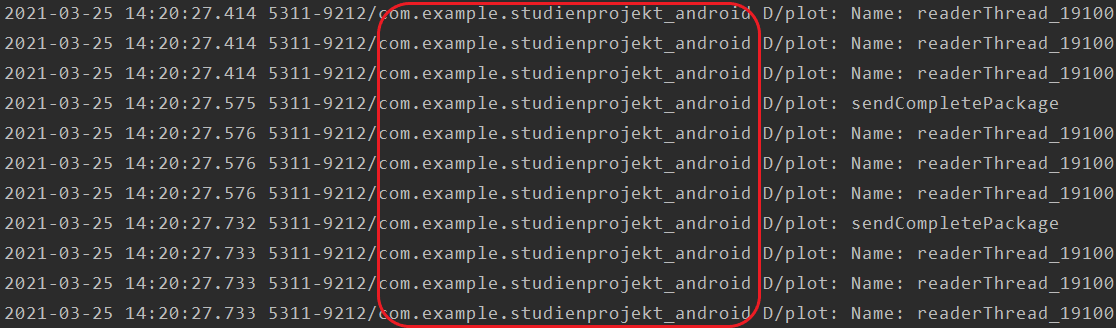
\includegraphics[width=0.8\textwidth]{Logcat_laufend.PNG}
	\caption{Logcatausgabe bei laufender App}
\end{figure}

\begin{figure}[htbp] 
	\centering
	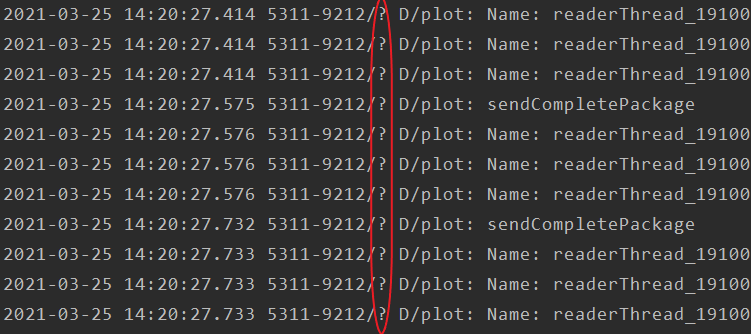
\includegraphics[width=0.8\textwidth]{Logcat_nichtLaufend.PNG}
	\caption{Logcatausgabe bei nicht laufender App}
\end{figure}

Dieses Problem liegt nicht daran, dass der readerThread nicht richtig beendet wird, wenn die App geschlossen wird, da ein Aufruf von „readerThread.interrupt()“ nicht hilft.\par
Wenn man die App deinstalliert und das Smartphone neu startet, dann wird bei Android Studio in Logcat nichts mehr ausgegeben. Deswegen wird empfohlen, wenn die App auf dem eigenen Smartphone ausgeführt wird, nach der Deinstallation das Smartphone neu zu starten. 

\begin{table}[H] 
	\centering
	\scalebox{0.9}{
	\begin{tabular}{!{\color{black}\vrule}c!{\color{black}\vrule}c!{\color{black}\vrule}} 
		\cline{1-1}\arrayrulecolor{black}\cline{2-2}
		Server-Version
		1.0 & Server-Version
		2.0                                                                                                                                                                         \\ 
		\arrayrulecolor{black}\cline{1-1}\arrayrulecolor{black}\cline{2-2}
		\multicolumn{2}{!{\color{black}\vrule}c!{\color{black}\vrule}}{\begin{tabular}[c]{@{}c@{}}Auflösung:			1260x625 \\Iterations:			50 \\Anzahl			Clients: 1 \\			Client-Typ:			Android \\Messung			1\end{tabular}}       \\ 
		\arrayrulecolor{black}\hline
		ca.
		300 Sekunden   & ca. 210 Sekunden                                                                                                                                                                              \\ 
		\hline
		\multicolumn{2}{!{\color{black}\vrule}c!{\color{black}\vrule}}{\begin{tabular}[c]{@{}c@{}}Auflösung:			500x500 \\Iterations:			50 \\			Anzahl			Clients: 1 \\Client-Typ:\\			Android			Messung			2\end{tabular}}      \\ 
		\hline
		nicht
		gemessen     & ca.
		70 Sekunden                                                                                                                                                                            \\ 
		\hline
		\multicolumn{2}{!{\color{black}\vrule}c!{\color{black}\vrule}}{\begin{tabular}[c]{@{}c@{}}Auflösung:			500x500 \\			Iterations:			200 \\Anzahl			Clients: 1 \\			Client-Typ:			Android \\Messung			3\end{tabular}}    \\ 
		\hline
		nicht
		gemessen     & ca.
		80 Sekunden                                                                                                                                                                            \\ 
		\hline
		\multicolumn{2}{!{\color{black}\vrule}c!{\color{black}\vrule}}{\begin{tabular}[c]{@{}c@{}}Auflösung:			1000x1000 \\Iterations:			200 \\Anzahl			Clients: 1 \\Client-Typ:			Android \\Messung			4\end{tabular}}        \\ 
		\hline
		nicht
		gemessen     & ca.
		165 Sekunden                                                                                                                                                                           \\
		\hline
	\end{tabular}
}

\end{table}

Messungen 2, 3 und 4 konnten bei der Server-Version 1.0 nicht gemessen werden, da man die Auflösung nicht anpassen konnte. Man kann allerdings gut erkennen, dass die benötigte Zeit von Server-Version 1.0 zu 2.0 stark reduziert wurde. Des Weiteren ist gut erkennbar, dass die Erhöhung der Iterations keine dramatischen Einfluss auf die Berechnungsdauer hat (Messungen 2 und 3), denn die benötigte Zeit hat sich im Gegensatz zur Iteration nicht vervierfacht. Einen viel größeren Einfluss auf die Zeit nimmt hingegen die größer der Auflösung (Messungen 3 und 4). Hier wurde jeweils die Höhe und die Breite verdoppelt, die Fläche wurde also vervierfacht, die benötigte Zeit hat sich circa verdoppelt.


\section{CUDA Client}
\subsection{Verwendete Technologie}
\subsection{Bedienungsanleitung}
\subsection{Entwicklung \& Probleme}

\section{JavaScript Client}
\subsection{Verwendete Technologie}
Die eigentliche Berechnung der Mandelbrotmenge erfolgt nicht durch JavaScript sondern durch WebAssembly, ein Format binärer Anweisungen für Stack-basierte Virtuellen Maschinen. Als portables Kompilierungsziel höherer Programmiersprachen ermöglicht es den Einsatz dieser in Webanwendungen.  Auf dieses Projekt bezogen bedeutet das also, dass die Mandelbrotmenge in einer Funktion berechnet wird, die ursprünglich in C++ geschrieben wurde, jedoch im Browser ausgeführt werden kann, was wiederum zu einer schnelleren Ausführung als unter einer Berechnung in JavaScript selbst führt. Dazu muss die Datei „mandelbrot.cpp“, welche die benötigte Funktion „plot“ beinhaltet, in das WebAssembly-Format übersetzt werden. Zu diesem Zweck wird das online Tool „WebAssembly Explorer“ verwendet, welches die C++ Datei zunächst in das .wat-Textformat kompiliert und schließlich in die benötigte .wasm-Datei im Byteformat konvertiert. \par
Der damit gewonnene WebAssembly-Code wird im Client daraufhin über die fetch-API geladen und kompiliert. Anschließend wird eine ausführbare Instanz aus dem geladenen WebAssembly-Modul erstellt, aus der die Funktion „plot“ mit den benötigten Parametern in eine JavaScript-Variable exportiert werden kann. Diese Variable beinhaltet also die Instanz mit der exportierten Funktion, die von nun an durch JavaScript im Browser ausgeführt werden kann.
Der Rest des Clients läuft auf Basis von JavaScript, was dementsprechend den Verbindungsaufbau mit dem Server sowie die Kommunikation mit diesem beinhaltet. Für diesen Zweck folgt der Client dem WebSocket-Protokoll, ein auf TCP basierendes Netzwerkprotokoll, welches eine Vollduplex-Verbindung zwischen dem Client und dem Server, welcher ebenfalls das WebSocket-Protokoll erfüllen muss, ermöglicht. \par
Zu Beginn der Verbindung müssen Client und Server einen sogenannten Handshake durchführen. Dazu sendet der Client eine Anfrage an den Server, die Verbindung zu einer WebSocket-Verbindung zu erweitern. Eine solche Anfrage sieht beispielsweise folgendermaßen aus: \\ \\
GET / HTTP/1.1 \\
Host: 169.254.108.186:5000 \\
Accept: */* \\
Accept-Language: de,en-US;q=0.7,en;q=0.3 \\
Accept-Encoding: gzip, deflate \\
Sec-WebSocket-Version: 13 \\
Sec-WebSocket-Extensions: permessage-deflate \\
Sec-WebSocket-Key: gc4QSLz27bBKbb9AG28/Yg== \\
Connection: keep-alive, Upgrade \\
Upgrade: websocket \\

Die wichtigsten Bestandteile dieser Anfrage sind der zufällig generierte Sec-WebSocket-Key und die Forderung, auf das WebSocket-Protokoll umzusteigen. Erreicht die Anfrage nun den Server, muss dieser eine Antwort in einem festgelegten Format versenden. Dafür liest der Server den Sec-WebSocket-Key aus der Anfrage und fügt den Globally Unique Identifier 258EAFA5-E914-47DA-95CA-C5AB0DC85B11 an diesen an. Aus dem dabei entstandene Schlüssel wird daraufhin der SHA-1 Hash berechnet, welcher anschließend Base64-codiert wird.  Der resultierende String wird daraufhin dem Sec-WebSocket-Accept Header hinzugefügt, wodurch die Antwort des Servers beispielsweise so aussehen würde: \\ \\
HTTP/1.1 101 Switching Protocols \\
Connection: Upgrade \\
Upgrade: websocket \\
Sec-WebSocket-Accept: YzNjMGJlYjBmMDRjZDFmZGE5NGI1ZjgwNGU3NDAxZjc4\\N2RjZThmNA== \\

Mit Versand dieser Antwort ist eine Verbindung zwischen Client und Server aufgebaut und der eigentliche Datenaustausch kann beginnen. Die Nachrichten, die zwischen Client und Server verschickt werden, sind jedoch codiert und müssen vom Server vor dem Lesen und Schreiben entsprechend decodiert, beziehungsweise codiert werden. Von besonderer Bedeutung sind bei dieser Codierung die Bits, die die Länge der Nutzdaten angeben, der Markierungsschlüssel und die Bits, die die Nutzdaten selbst beinhalten. \par
Um die Länge der Nachricht zu ermitteln, liest der Server die Bits 9-15 und interpretiert diese als unsigned integer. Ist diese Zahl kleiner gleich 125, so ist sie die Länge der Nachricht. Ist sie 126, so müssen die nächsten 16 Bit als unsinged integer interpretiert werden, um die Länge zu ermitteln, und ist sie 127, so sind es die nächsten 64 Bit. Auf die Länge folgen nun 32 Bit, in denen sich der Maskierungsschlüssel befindet. Anhand dieser Informationen kann die Nachricht nun decodiert werden, indem Byte für Byte durch die codierte Nachricht iteriert und auf diese den XOR-Operator mit dem  Byte des Maskierungsschlüssel an der Stelle (i\%4) angewendet wird.  Analog zu diesem Verfahren codiert der Server Nachrichten, bevor er sie an den Client verschickt, und er somit das WebSocket-Protokoll vollständig umsetzt, wodurch eine Kommunikation mit WebSocket-Clients möglich ist.\\

\subsection{Bedienungsanleitung}
\subsubsection{Vorbereitung des Browsers}
Da es im Browser zu einem Cross-Origin Ressource Sharing (CORS) Error führen kann, wenn der JavaScript-Client versucht, das WebAssembly-Modul zu laden, müssen zu dessen Ausführung Einstellungen geändert werden. \\
Mozilla Firefox: 
\begin{enumerate}
	\setlength\itemsep{0.07em}
	\item In die Suchleiste des Browsers „about:config“ eingeben und bestätigen.
	\item Den Knopf „Risiko akzeptieren und fortfahren“ anklicken.
	\item In die Suchleiste „origin“ eingeben.
	\item Den Eintrag „privacy.file\_unique\_origin“ von true auf false setzen.
	\item Den Browser schließen und neustarten.
\end{enumerate}
Da hiermit Einstellungen verändert werden, empfiehlt es sich, nach Beenden der Berechnung diese wieder zu reversieren.
\subsubsection{Verwendung des Clients}
\begin{enumerate}
	\setlength\itemsep{0.07em}
	\item Sicherstellen, dass die Dateien „js\_client.html“ und „mandelbrot.wasm“ im selben Verzeichnis liegen.
	\item Den Server starten und die auf der Konsole ausgegebe IP und den Port kopieren.
	\item Die Datei „js\_client.html“ mit einem Textbearbeitungsprogramm öffnen und die Variablen „ip“ und „port“ in den Zeilen 25 und 26 anpassen und die Datei speichern.
	\item Die Datei „js\_client.html“ im Browser öffnen.
	\item Gegebenenfalls die Konsole öffnen und überprüfen, ob der Client Aufträge entgegen genommen hat. Wenn nicht, die Seite neu laden, bis Aufträge erfolgreich entgegen genommen werden, und die Konsole schließen.
\end{enumerate}
\subsection{Entwicklung \& Probleme}
Nach der Auswahl von JavaScript mit WebAssembly zur Ergänzung als die Technologie für diesen Client war der erste Schritt, erst die Funktionsweise von WebAssembly kennenzulernen. Entsprechend war die erste Erwartungshaltung, dass die Entwicklung von WebAssembly-Modulen und deren funktionierende Einbindung in JavaScript, den kompliziertesten Teil der Cliententwicklung ausmachen würden. Daher entsteht zunächst ein kurzes Programm in C++, welches die Fakultät einer übergebenen Zahl berechnet und in den Client eingebunden wird. \\
Über Konsoleneingaben und –ausgaben wird die Funktionalität erfolgreich getestet. Da die spätere Einbindung einer Funktion, die die Mandelbrotmenge berechnen soll, analog geschehen würde, ist die Verbindung zwischen Server und Client der nächste Schritt in der Entwicklung. \par

Der erste Punkt, der sich als Problem herausstellt, ist die Tatsache, dass normale TCP Sockets, wie sie beispielsweise in dem Client unter Android oder Cuda verwendet werden, mit JavaScript nicht kompatibel sind. Daher muss eine Verbindung unter den oben genannten WebSocket geschehen, einer Technologie, in die sich ebenfalls zuerst eingelesen werden musste. Da am Anfang noch kein gemeinsamer Server besteht, auf den alle drei verschiedenen Arten von Clients zugreifen können, erfolgt der erste Verbindungstest mit einem kleinen Testserver, der in Node.js geschrieben ist. Die Wahl fällt dabei auf Node.js, da der Server somit genau wie der Client in JavaScript geschrieben werden kann und somit ohne Einbindung externer Bibliotheken von sich aus das WebSocket-Protokoll unterstützt. Zu Testzwecken werden Zahlen vom Testserver an den Client geschickt, der aus diesen mithilfe des eingebundenen WebAssembly-Moduls die Fakultät berechnet und sie daraufhin an den Server zurück sendet. Damit ist sichergestellt, dass der Client sich sowohl mit einem WebSocket-kompatiblen Server verbinden kann als auch Daten von diesem empfangen, die Daten per WebAssembly-Funktionen verarbeiten und sie an den Server zurück schicken kann. \par

Im nächsten Schritt beginnt die Entwicklung des eigentlichen Servers für das Projekt, für den sich auf Java als Programmiersprache geeinigt wurde. Da Java von sich aus WebSocket-Verbindungen nicht ohne weiteres unterstützt, wurde zunächst nach einer Bibliothek oder API für Java gesucht, die eine solche Verbindung ermöglichen könnte. Allerdings existieren lediglich APIs, die die Verwendung von Jakarta EE voraussetzen, weswegen die manuelle Umsetzung des WebSocket-Protokolls für den gemeinsamen Server, der in der Java Platform, Standard Edition geschrieben ist, von Nöten ist. \par

Um die Verbindung zwischen WebSocket-Client und Server überhaupt erst ermöglichen zu können, muss der Server in der Lage sein, eine eingehende Anfrage für einen Handshake zu erkennen und daraus die Verbindung zu genau diesem Client, der die Anfrage geschickt hat, zu einer WebSocket-Verbindung zu erweitern. Zwar erweist sich der eigentliche Vorgang des Handshakes und der Antwort auf diesen als relativ unkompliziert, so führt es aber zu einem Problem, wenn die Art des sich zu verbindenden Clients nicht vor Ausführung des Handshakes ermittelt wird. So wird bei erfolgreicher Ausführung des Handshakes zwar eine erfolgreiche Verbindung zwischen dem Server und dem auf WebSockets basierendem Client aufgebaut, erfolgt der Handshake allerdings bedingungslos für jeden Client, so sind die Clients, die auf regulären TCP-Sockets basieren, daraufhin nicht mehr in der Lage, Nachrichten mit dem Server auszutauschen. Eine Erkennung des Client-Typen ist also zwingend erforderlich. \par

Die erste Idee ist es, dass jeder Client nach Aufbau der Verbindung als erste Nachricht seinen eigenen Typen an den Server sendet. So soll nur im Fall der Nachricht „type/.WebSocket“ der Handshake und damit die Aufwertung auf eine WebSocket-Verbindung erfolgen, die anderen beiden Typen von Clients bleiben damit also unberührt. Diese Umsetzung scheitert an der Tatsache, dass ein WebSocket-Client keine Nachrichten mit dem Server austauscht, ehe der Handshake getätigt wurde. Die erste Nachricht, die der Server von einem WebSocket-Client erhält, ist also „GET / HTTP/1.1“, die erste Zeile der Handshake-Anfrage. Stattdessen überprüft der Server daher, ob ein Client eine Nachricht gesendet hat, die auf „type“ beginnt und falls nicht, werden die restlichen Zeilen der Handshake-Anfrage eingelesen,  an die erste Zeile gehangen und der Handshake erfolgreich durchgeführt. Ab diesem Punkt sind sowohl TCP-basierte Clients als auch WebSocket-Clients in der Lage, eine Verbindung zum Server aufzubauen. \par

Mit einer erfolgreichen Verbindung zum Server kann der Client nun beginnen, Nachrichten an den Server zu schicken. Mit der ersten verschickten Nachricht offenbart sich bereits aber das nächste Problem. Die vermeintlichen Nachrichten vom Client, die der Server ausgibt, bestehen vollständig aus Unicode Ersetzungszeichen. Da sämtliche Nachrichten, die der WebSocket-Client nach Abschluss des Handshakes an den Server sendet, codiert sind, genügt es demnach nicht, auf Seite des Servers den InputStream zu lesen und die dort eingehenden Zeichen als einen vollständigen String zu interpretieren. \par

Stattdessen handelt es sich um Bytes, die nach oben genannter Vorgehensweise decodiert werden müssen. Der Server liest die Länge der Nachricht und den Maskierungsschlüssel aus den Bytes und verwendet diese Informationen, um aus den darauf folgenden Bytes die eigentliche Nachricht zu decodieren. Die erste Implementierung berücksichtigt zunächst keine Nachrichten, die über mehrere Lesevorgänge verteilt sind, was bei langen Nachrichten zu Problemen führt, da sie zum Teil nicht vollständig decodiert werden und es zu Formatierungsfehlern kommt, wenn diese zum Beispiel in einen int-Wert konvertiert werden sollen. Zu diesem Zweck überprüft der Server, ob die Zahl der gelesenen Bytes tatsächlich denen der vorgesehen Länge entsprechen und falls nicht, wird im nächsten Lesevorgang die Nachricht an entsprechender Stelle erweitert. Dennoch werden nicht unter allen Umständen sämtliche Nachrichten korrekt gelesen. Unter einer hohen Anzahl an eingehenden Nachrichten geschieht es, dass einige von ihnen als leerer String interpretiert werden. \par

Aufgrund der Notwendigkeit der Codierung unter WebSockets tritt beim Verschicken von Nachrichten vom Server zum Client ein sehr ähnliches Problem auf. Anstatt nicht entzifferbarer Ersetzungszeichen erreichen den Client jedoch gar keine Nachrichten. Demensprechend müssen die Nachrichten, die der Server an den Client schickt, zuvor ebenfalls codiert werden. Nach einer Codierung als Byte-Array gemäß dem WebSocket-Protokoll, können die Nachrichten durch einen DataOutputStream an den Client verschickt werden. Die Art des OutputStreams ist daher von Bedeutung, da unter Verwendung eines gewöhnlichen OutputStreams keine Nachrichten vom Client erkannt werden, als seien sie nicht codiert worden. \par

Mit der funktionierenden Kommunikation zwischen Server und Client kann der Server nun Aufträge an den WebSocket-Client versenden und unter Verwendung von WebAssembly das Ergebnis der Mandelbrotmenge für diese Aufträge errechnen und zurücksenden. Da in sämtlichen dieser Schritte Strings verarbeitet werden und der Umgang mit diesen grundsätzlich langsamer ist als das Verschicken und Verarbeiten von Byte-Arrays, erfolgt ein Versuch, die Aufträge als Byte-Arrays zu übergeben. Dieser Versuch scheitert an zwei Problemen: Sämtliche Nachrichten werden bereits als Byte-Arrays verschickt, die Codierung ist aber auf Strings als Ergebnis ausgedacht, sodass der Client von den Aufträgen fast ausschließlich Ersetzungszeichen erhält. Zudem kommt es zu einem Verbindungsabbruch von Seiten des Clients, auf den der Server aber nicht reagiert. Das führt zu einem SocketWriteError, da nur einseitig die Verbindung getrennt wird und der Server versucht, über einen nicht mehr belegten Socket wiederholt „noTask“-Nachrichten zu versenden. Aufgrund dieser Probleme verarbeiten sowohl Client als auch Server weiterhin Strings, auch wenn das einen potenziellen Zeitverlust bedeutet. \par

Die Einbindung eines funktionierenden WebAssembly-Moduls zur Berechnung der Mandelbrotmenge erweist sich als unproblematisch, jedoch zeigen sich bei der Art und Weise, wie die berechneten Ergebnisse an den Server gesendet werden, weitere Probleme. So verschickt der Client in der ersten Version für jeden abgearbeiteten Bildpunkt eine „plot“-Nachricht, um den Server darauf hinzuweisen, dass als nächstes die errechneten Werte folgen, in drei separaten Nachrichten den x-Wert, den y-Wert und den errechneten Iterationswert und anschließend an die vollständige Berechnung des Auftrags jeweils eine „tick“-Nachricht, um den Server aufzufordern, das Bild zu rendern, und eine „task“-Nachricht, um den nächsten Auftrag anzufordern. Bei einer Bildbreite von 500 Pixeln ergibt das also 2002 Nachrichten pro berechneten Auftrag. \par

Da der Server diese Anzahl an Nachrichten nicht korrekt decodieren kann, ist die zuvor genannte Anpassung, dass Nachrichten über mehrere Lesevorgänge eingelesen werden müssen notwendig. Zwar werden mit dieser Variante keine falschen Zeichen mehr ausgegeben, jedoch werden Nachrichten zufällig als leerer String interpretiert, was einen Informationsverlust bedeutet, der zu schwarzen Flecken auf der gerenderten Mandelbrotmenge führt. \par

\begin{figure}[htbp] 
	\centering
	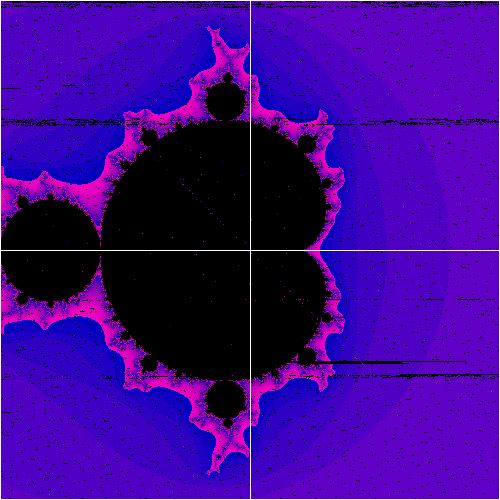
\includegraphics[width=0.5\textwidth]{einzelnVersandt.PNG}
	\caption{Mandelbrotmenge bei separatem Versand jedes einzelnen Wertes}
	\label{fig:Bild1}
\end{figure}

Um überhaupt das Bild rendern zu können, werden leere Nachrichten ignoriert und stattdessen versucht, mithilfe von vorhandenen Informationen wie dem fortlaufenden x-Wert oder dem y-Wert der berechneten Werte, der sich bei einem Auftrag nicht mehr ändert, diese zu rekonstruieren. Der verlorene Iterationswert hingegen kann aus diesen Daten nicht erfasst werden und soll durch den zuvor berechneten Iterationswert ersetzt werden. Da es sich dabei also nicht für jeden Punkt um den korrekt berechneten Iterationswert handelt, ist das entstehende Bild lediglich eine Approximation der Mandelbrotmenge. Dennoch entstehen eine Vielzahl an schwarzen Flecken auf der Graphik sowie falsch gesetzte Ersatzpixel. Das ist damit zu erklären, dass es nicht garantiert ist, dass auf eine verlorene Nachricht wieder eine korrekt erfasste Nachricht folgt. Somit können mehrere Nachrichten hintereinander verloren gehen, worauf dieser Ausgleichmechanismus nicht ausgelegt ist. \par

Ebenfalls erweist sich die Zeiterfassung für diese Methode der Datenübertragung als schwer. Der Client beendet seine Berechnung scheinbar wahllos und muss neu gestartet werden, um weiterhin Bildpunkte zu berechnen. Erst mit einer Konsolenausgabe, dass ein Auftrag fertig berechnet wurde, zeigt sich, dass der Client immer nach Beenden eines Auftrages anhält und keine weiteren Aufträge mehr erhält. Das lässt sich damit erklären, dass auch die Nachricht, mit der der Client neue Aufträge anfordert, vom Server als leerer String interpretiert werden kann und die Berechnung somit zum Halt kommt. Lädt man den Client neu, sobald er aufhört, Punkte zu berechnen, dauert die gesamte Darstellung der Mandelbrotmenge lokal ca. 4 Minuten; ein Wert der aufgrund des wiederholten, manuellen Ladens des Clients ungenau ist.\par

Der Versuch, sämtliche berechneten Punkte durch Zeilenumbrüche getrennt in einer Nachricht zu verschicken, scheitert daran, dass die Nachricht zwar korrekt vom Server gelesen wird, jedoch in der Funktion, in die der String übergeben wird, als null-String ausgegeben wird. Daher ist der nächste Schritt, diese Zeilen einzeln zu versenden. So werden x-Wert, y-Wert und die berechnete Iteration eines jeden Bildpunkts jeweils mit einem Trennzeichen zwischen aneinander gekettet und verschickt. 

\begin{figure}[htbp] 
	\centering
	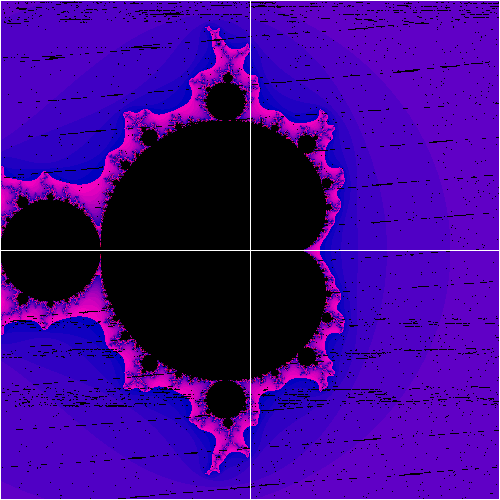
\includegraphics[width=0.5\textwidth]{zeilenVersandt.PNG}
	\caption{Mandelbrotmenge bei separatem Versand jedes einzelnen Punkts}
	\label{fig:Bild2}
\end{figure}

Da auch auf die „plot“-Nachricht vor dem Versenden der Ergebnisse verzichtet werden kann, reduziert sich die Anzahl der Nachrichten damit bei einer Bildbreite von 500 Pixeln also von 2002 Nachrichten auf 502 Nachrichten.\\
Doch auch bei dieser Variante werden Nachrichten vom Server als leere Strings interpretiert und schwarze Punkte auf der Graphik gesetzt. Erneut erweist sich die Zeiterfassung als schwierig, da die Auftragsanfrage ebenfalls vom Server fehlinterpretiert werden kann, wenn auch seltener als in der zuvor verwendeten Version. Mit diesem ungenauen, manuellen Wiederverbinden des Clients einbegriffen dauert die Darstellung der Mandelbrotmenge bei dieser Variante lokal ca. 70 Sekunden, was im Vergleich zu der ersten Variante einen Geschwindigkeitsgewinn darstellt. Ebenfalls lässt sich eine gewisse Regelmäßigkeit im Vergleich zu den schwarzen Punkten der ersten Variante feststellen. So scheinen die schwarzen Punkte beim zeilenweisen Versenden der Ergebnisse  diagonale Linien auf der Graphik zu ziehen. Die irregulären Anhäufungen von schwarzen Punkten geschehen hingegen immer dann, wenn der Client neugeladen werden muss. \par
Da der Server mit 502 Nachrichten pro Auftrag noch nicht in der Lage ist, sämtliche eingehende Nachrichten korrekt zu decodieren, gleichzeitig aber auch keine 500 Zeilenumbrüche in einem String verarbeiten kann, werden die Ergebnisse in der finalen Version alle in einem String pro Auftrag verschickt. Das reduziert die Anzahl der versendeten Nachrichten pro Auftrag unabhängig von der Bildbreite auf 3: eine „plot“-Nachricht, die Ergebnisse und eine Aufforderung, das Bild zu rendern. Um zu verhindern, dass keine Aufträge mehr verschickt werden und die Berechnung anhält, verschickt der Server nun selbstständig einen neuen Auftrag an den Client, sobald dieser einen abgearbeitet hat. Auf diese Weise werden keine Nachrichten mehr als leere Strings interpretiert und somit die Mandelbrotmenge vollständig angezeigt. Lokal berechnet dauert das Darstellen der Startkonfiguration in der finalen Variante bei den Maßen 500 x 500 durchschnittlich 2.4 Sekunden.\par

Doch auch in der finalen Variante kann es dazu kommen, dass Nachrichten vom Server als fehlerhafte Zeichen interpretiert werden, was zu einer NullpointerException führt. In diesem Fall wird der Auftrag, für den die Ergebnisse erwartet werden, zurück in die Liste der Aufträge geschrieben und ein neuer Auftrag an den Client vergeben. Wenn jedoch mehrere Nachrichten und damit mehrere Reihen hintereinander vom Server als eine einzige Nachricht fehlinterpretiert werden und damit nur der erste Auftrag zurück in die Liste geschrieben wird, können vollständige Reihen in der Graphik verloren gehen. Während dieser Fehler bei der lokalen Verwendung des Clients bei den Standardmaßen extrem selten ist, wird er bei großer Breite des Bildes häufiger und tritt bei der Verbindung zu einem nicht-lokalen Server stets auf.


\section{Server}


\section{Reflexion}


\nocite{*}




\end{document}

